\chapter{Further analysis and discussion}

This chapter aims to analyse and discuss the findings presented in the previous three chapters, focusing on the intricate details and implications of Atomic Force Microscopy (AFM) force curve analysis. The preceding chapters laid a foundational understanding of the colloidal interactions and the work involved to process the raw data into a usable format. This chapter instead will focus on using the previous chapters' data to draw conclusions about colloidal systems. The force-distance profiles obtained from AFM are analysed, providing a direct and nuanced insight into the particle interactions at an individual level. The force curves, reflecting the precise nature of forces acting at the nanoscale, will be juxtaposed against the bulk property measurements to draw a more comprehensive picture of the colloidal dynamics. This analysis will not only validate but also potentially challenge and refine the conclusions drawn from the bulk measurements, offering a more holistic understanding of the colloidal systems under study. Through this integrative approach, we aim to bridge the gap between our microscopic observations and derive behaviour on the macro scale. This chapter takes the following format, firstly over viewing the approach data, then the retract data.

\section{Approach force curves}

The approach curve section of the data demonstrated a range of interesting effects and features. For one, the increase in LiCl concentration directly resulted in a decrease of the repulsive force upon the tip, likely due to the charge screening effect. At certain concentrations (550mM) this repulsive force flips into an attractive force, presumably where the electrostatic repulsion was muted enough for Van der Waals forces to predominate. However, even then, there was a notable range of attractive force, with some 550mM curves having very little attraction (550mM site 2). 

The variety in the magnitude of attractive forces at this high ionic strength, especially observed in the 550mM site 2 curves, further complicates the narrative. Such variability could be the result of surface heterogeneity, variations in ion distribution, or differing hydration layers, each of which could alter the force profile significantly.

Another interesting feature observed is the shelf. This shelf presented a sometime present energy barrier for the tip to overcome to come into contact. The presence of this shelf could possibly influence the plateau seen in the Averaged Approach Force vs LiCl Concentration graph, as the script was set to define contact as after the shelf.

Interestingly, the absence of a shelf often correlated with lower repulsive forces, suggesting a relationship between the energy barrier and the overall force profile. In the case of 550mM concentrations, where an attractive force towards the surface was noted, the presence of an energy barrier despite the attraction further adds to the complexity. It raises questions about the nature of these barriers: whether they are purely electrostatic or if other forces, such as steric or hydration forces, contribute to their formation.

\section{Retract force curves}

The retract force curves, which are often omitted due to their lack of acquiescence to DLVO, have several interesting properties too. Firstly, in general as the LiCl concentration increases, so too does the attractive force between the surface and the tip. But equally, when dwell time is applied, the attractive force additionally increases. This likely means that the mechanism holding the tip down during retrace may be dependant on ionic effects.

When dwell time is factored in, the attractive force further increases. This increment is indicative of a time-dependent process, possibly due to the reorganization of ions around the contact point, which enhances the attractive forces. The mechanism underlying this could be attributed to a combination of factors such as ion adsorption, water structuring, or surface conditioning over time, which requires further investigation.

The increasing attraction with dwell time also underscores the dynamic nature of colloidal interactions, where the history of contact and the duration of interaction significantly influence the force profiles. This temporal aspect is often not captured in instantaneous measurements and suggests a viscoelastic or time-dependent response in the colloidal system.

In addition, the retract force curves with varying LiCl concentrations provide insights into the complexity beyond what is described by classical DLVO theory. The increased attraction at higher ionic strengths contradicts the expected screening effect that should reduce the interaction forces. This anomaly could be hinting at non-DLVO interactions, such as capillary forces, hydrophobic interactions, or specific ion effects, which are not accounted for in the classical theory.

Additionally, there are some curiosities in the dataset, 25mM for example has a dramatic spike in attractive force towards the surface. This is further compounded by the dwell time decreasing the attractive force for 25mM. The shelf feature, as seen in the approach curves, is also present in the retract curve, indicating that the energy barrier may be more akin to an energy trap, which could lead towards the potential of surface roughness/frictional forces between the tip and surface.

\section{Shelf analysis}

The shelf seen in some datapoints is a consistent feature across multiple sites, present in the majority of the curves. The only concentration that doesn't feature the shelf in any of the sites is the 0.6mM concentrations, which is equally true in both the MFP and JPK AFMs.

However the shelf was also seen in the JPK forcemaps as well - specifically the 10mM curves. Though, the shelf prominence varies between sites, some have a visible shelf that extends across multiple nanometers, while others don't. This feature is also seen in other papers from literature.\cite{guleryuz2012afm}

However, it is prudent to ensure that the script is not the cause of this feature. As part of the curve is used to align the data into a straight line for the contact region, it is conceivable that this was introduced by the user defining said region.

\begin{figure}[h!]
\centering
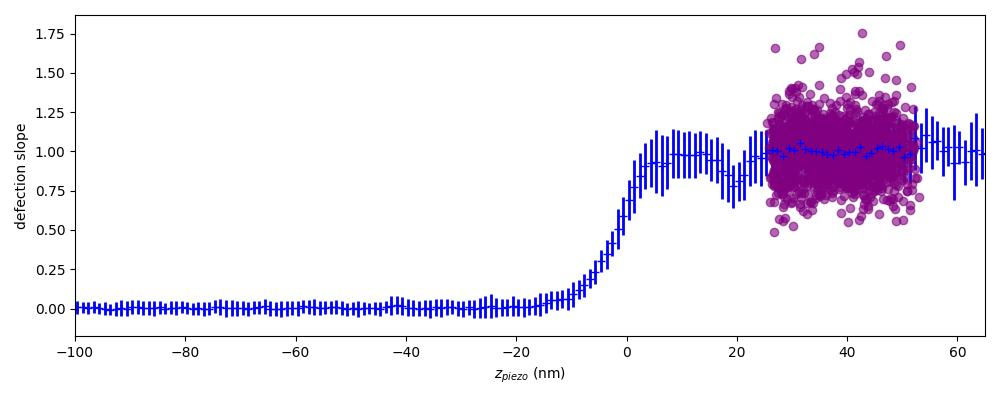
\includegraphics[width=0.8\textwidth]{chapter8/Shelf/Post 1.6 S4 df_deriv_bin.jpg}
\caption{An example of a derived deflection slope vs z separation processed curve. This curve is used to help guide the user to optimise the fitting parameters. The purple region indicates the region used to define contact, and to help straighten the contact region.}
\label{fig:Deriv1}
\end{figure}
\begin{figure}[h!]
\centering
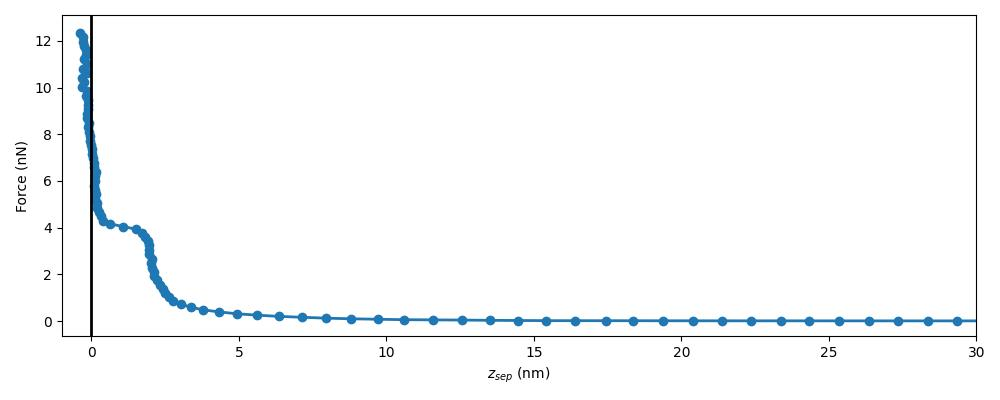
\includegraphics[width=0.8\textwidth]{chapter8/Shelf/Post approach_force_sep.jpg}
\caption{The fitted curve from the values above. The back is relatively straight.}
\label{fig:CurveBack}
\end{figure}

From Figure \ref{fig:Deriv1} and \ref{fig:CurveBack} the fit can be seen to be right after the shelf shift. This is intentional during the fitting process - as to fit closest to the transition point. However, to ensure that the feature isn't caused by the script, lets apply the contact point to the shelf itself.

\begin{figure}[h!]
\centering
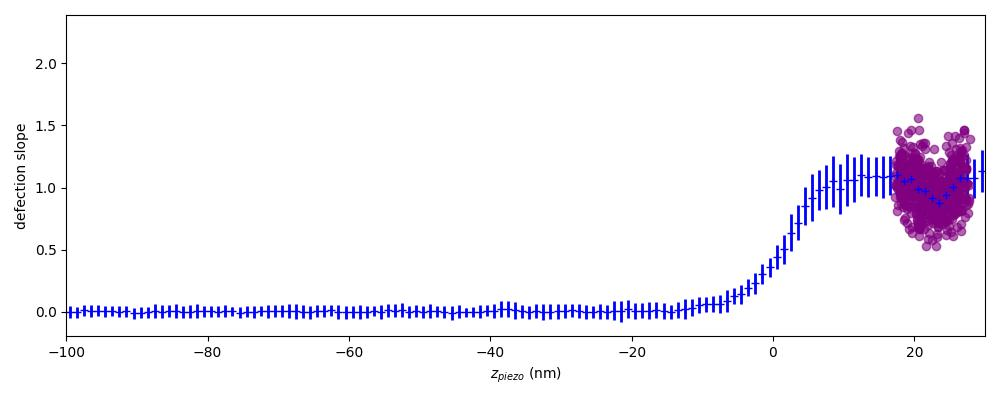
\includegraphics[width=0.8\textwidth]{chapter8/Shelf/Targeted df_deriv_bin.jpg}
\caption{An example of a derived deflection slope vs z separation processed curve. The purple region indicates the region used to define contact, and has specifically been placed onto the shelf area.}
\label{fig:Deriv2}
\end{figure}
\begin{figure}[h!]
\centering
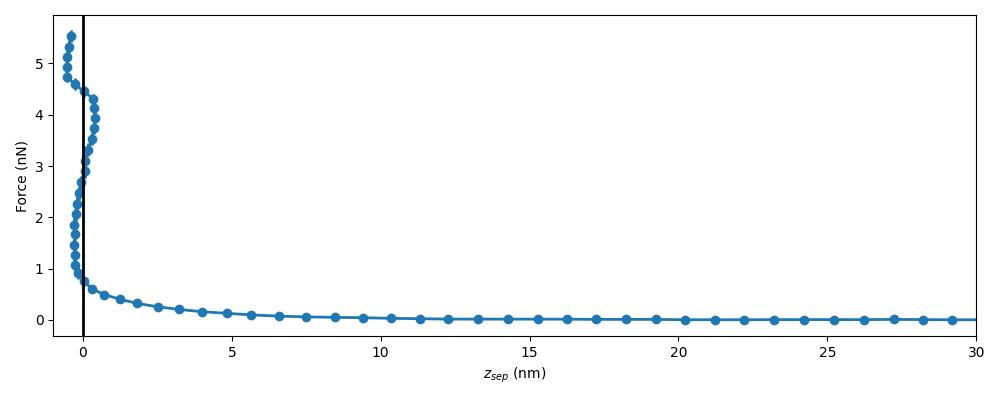
\includegraphics[width=0.7\textwidth]{chapter8/Shelf/Targeted approach_force_sep.jpg}
\caption{The fitted curve from the values above. The back is wonky, but the shelf feature prevails.}
\label{fig:CurveBack2}
\end{figure}

Figures \ref{fig:Deriv2} and \ref{fig:CurveBack2} demonstrate that the fitting does not influence underlying features of the graphs. The shelf is still present in the curves, and the shelf is at the same expected force.

One specific paper describes an attractive force that is observed when using a counterion at intermediate salt concentrations. This force has a range of about 1 nm and is distinct from the forces predicted by DLVO theory. It is believed that this additional force could be due to ion-ion correlations, which are interactions that can occur between ions in solution due to their charge. However, the shelf could also be influenced by other factors such as surface charge heterogeneities (variations in the distribution of charge on the surface) or charge fluctuation forces (forces that arise from temporary changes in the distribution of charge). \cite{Valmacco2016}

However one interesting point about the findings in that paper is the notation of a roughly 1 nm range. Given that several of the graphs in the dataset feature shelves, an analysis of the shelf force (the force required for the energy barrier to yield) and an analysis of the shelf range (the width of the shelf as seen on the dataset) would serve as a useful exploration for determining overlaps between our data and theirs.

\begin{figure}[h!]
\centering
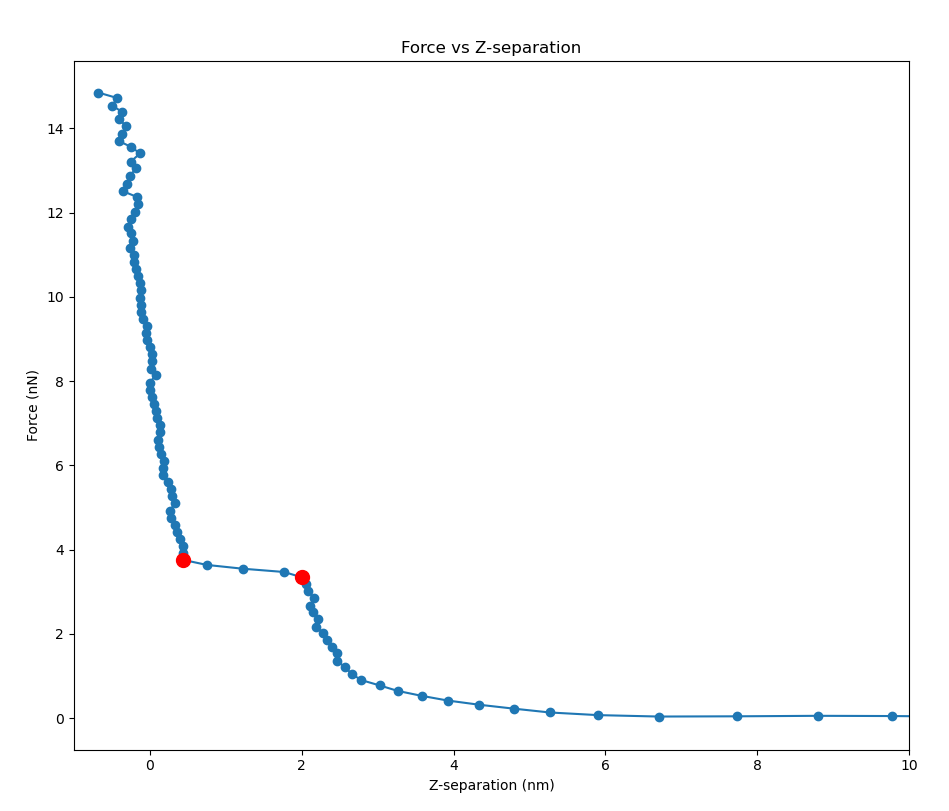
\includegraphics[width=0.45\textwidth]{chapter8/Shelf/Force calculatio.png}
\caption{Demonstrating the fitting range for the shelf analysis. The two red dots highlight the end points of the range. The shelf force is calculated by the average force for the points within the range, and the shelf range is calculated by the width of the two points in nm.}
\label{fig:forcecalc}
\end{figure}

This data was taken for all datapoints that could be extracted this way (one or two shelves were omitted due to the inability to define a firm range, i.e. the repulsive curve blended into the shelf feature, a good example of this is 25mM site 3). These points were then plotted in figure \ref{fig:resultsShelf}.

\begin{figure}[h!!]
\centering
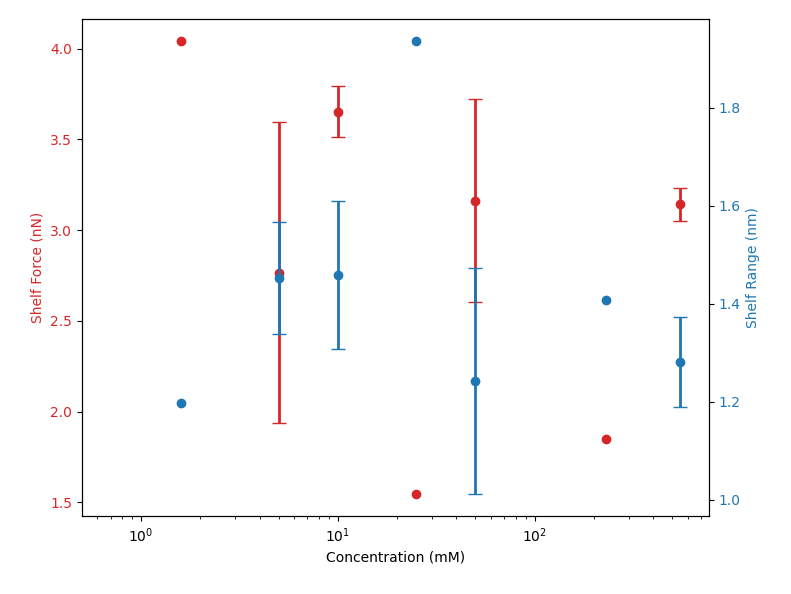
\includegraphics[width=0.8\textwidth]{chapter8/Shelf/ShelfScatter2.png}
\caption{Demonstrating the range of self force and self range. For the range of data, there was no significant change in the datapoints due to salt concentration for both features.}
\label{fig:resultsShelf}
\end{figure}

The results in \ref{fig:resultsShelf} show that the shelf had a consistent range between 1-2nm, and the yield force was between 1.5-4nN. While the range was slightly higher in our data, our findings align with what Kilpatrick et al discusses \cite{Kilpatrick2013DirectlyProbing}. The fact that the shelf is consistent across a broad range of salt concentrations might imply that these additional forces are present regardless of ionic strength variations, possibly due to surface charge heterogeneities or charge fluctuation forces that are less sensitive to ionic strength.

In addition to this finding, the JPK forcemapping curves demonstrated the same shelf seen across the standard dataset. As the tip moved across multiple locations, the shelf force changed, however the shelf range was relatively static.

\begin{figure}[h!!]
\centering
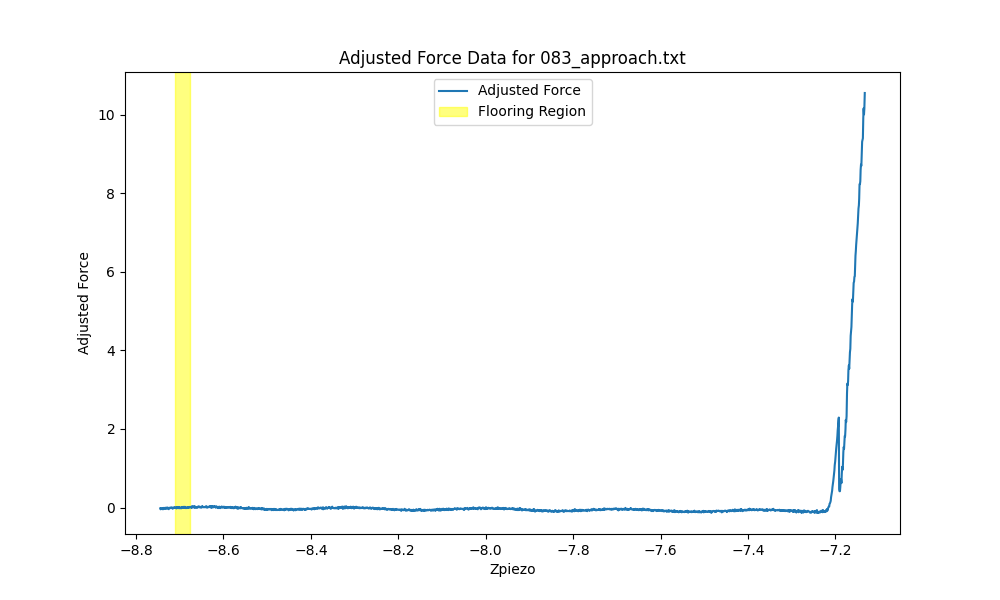
\includegraphics[width=0.8\textwidth]{chapter8/Shelf/083_approach.png}
\caption{An example of an unprocessed curve (except force flooring) from the JPK forcemapping. The "shelf" can clearly be seen, with a sudden jump down to contact. The difference between this and the MFP could be due to the higher resolution the newer AFM offers.}
\label{fig:noisey}
\end{figure}

One interesting aspect of this shelf as seen in the JPK AFM is the sudden attractive force felt by the tip. This again is in line with Kilpatrick et al.

As such our findings match Kilpatrick et al. \cite{Kilpatrick2013DirectlyProbing}, where the shelf can be attributed to additional, non-DLVO attractive forces likely related to the specific ion effects, such as ion-ion correlations, surface charge heterogeneities, or other surface-specific interactions at the water-silica interface such as hydration forces. These forces can be significant in the presence of multivalent ions, which are known to impact the surface charge and hydration layers in a manner not fully accounted for by classical DLVO theory. As such, this provides evidence towards a growing call for improvements to the current DLVO theory.

\section{Overcoming the noise in data}

The noise in the data from MFP AFM is significant. Not all AFMs can be operated in optimal conditions such as AFMs isolated from vibrations, under peak maintenance, free from external factors, etc. Other sources of noise in AFM can stem from electronic components, particularly those involved in the detection system, such as photodiodes and amplifiers. This includes shot noise from random electron motion, Johnson noise related to thermal motion within resistors, and noise intrinsic to operational amplifiers. Additionally, mechanical vibrations and thermal fluctuations also contribute to noise, affecting the spatial and temporal resolution of measurements. \cite{gittes1997signals}

\begin{figure}[h!]
\centering
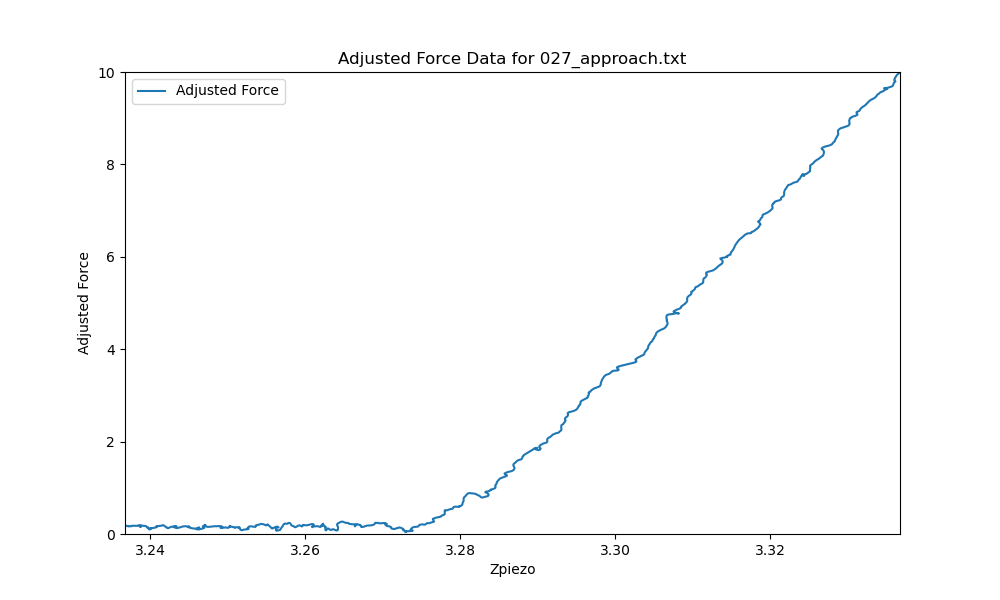
\includegraphics[width=\textwidth]{chapter8/Shelf/027_approach_zoom.png}
\caption{An example of a zoomed in portion of a raw curve. The noise is intense. The shelf feature can be somewhat seen in the curve, but could easily be discounted by the background noise.}
\label{fig:noisey}
\end{figure}

These sources of noise could have impacted the resulting graphs from the age of the components in the system. Other sources of noise and frustration during the data taking process is due to the variability in the force feedback loop. It was observed that the AFM doesn't always apply consistent pressure, especially during the dwell time graphs, which was the source of difficulty during their processing. The data rate as well as the limited amount of binning that could possible be done, as features would be lost/smoothed out. 

In science there is a constant pressure to use newer equipment, when older equipment is still potentially suitable. Given that newer AFMs can brush up against the million pound mark, it is imperative to consider whether the trade-offs justify such investments. The challenge with older instruments, is that the wear and tear over time can exacerbate the inherent noise issues. Components such as piezoelectric scanners, which are responsible for the precise movements required for imaging and force measurements, may degrade in performance, leading to drifts or instability in the collected data. Similarly, older detection systems may not be as effective in filtering out noise or may not have the same sensitivity as modern instruments.

However, the fundamental mechanics of AFM have remained relatively consistent, the primary mechanisms of force detection and image resolution are still based on the deflection of a cantilever and the distance control between the probe and the sample. Hence, an older, well-maintained AFM can still provide valuable data, particularly for applications where ultra-high resolution is not mandatory.

The software developed during this investigation provides a powerful tool for older AFMs, particularly for nosier systems. The ability to resolve the shelf feature is a significant one, as the baseline noise present in the MFP curves often hide the feature. This capability is seen throughout all of the variability in conditions seen throughout the various different sites. By utilising the scripts and methods used in this investigation, it opens up the possibility for the scientific community to extend the lifespan of older equipment, making it viable for current and future research without the immediate need for costly upgrades.

The scripts and analysis methods developed as part of this research cater to the nuanced intricacies of noise in AFM data, enabling the extraction of meaningful results even from signals that might be considered too noisy or from data that would otherwise be discarded. This notion is particularly relevant in the context of educational institutions and research facilities with limited funding, where such software enhancements can democratize access to high-quality research opportunities. 

\begin{figure}[h!]
\centering
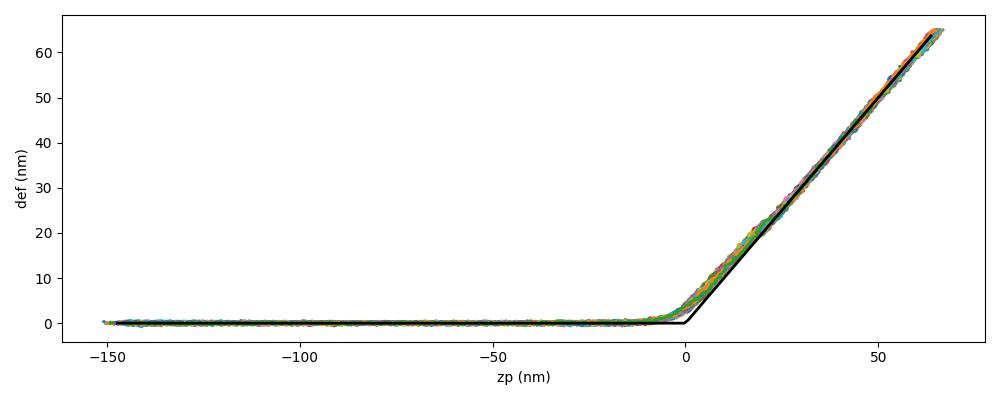
\includegraphics[width=\textwidth]{chapter8/Shelf/Post 1.6 S4 df_zp.jpg}
\caption{An example of an adjusted and overlapped portion of multiple curves. The shelf is clearly visible and highlighted throughout the multiple movements throughout the noise floor.}
\label{fig:noisey}
\end{figure}

The software utilises several methods of adjusting the curves towards a more user readable graph, without impacting the underlying data, this is in addition to binning the data to reduce the noise floor, while keeping binning rates sensible to retain the features of the curve. The sum effects of the software can be clearly seen in the extraction of the shelf features, which have previously been observed in literature \cite{Kilpatrick2013DirectlyProbing}, from otherwise convoluted curves. %DO NOT FORGET MEEEEE

By making this software open source and accessible on a git repository, the scientific community can utilise, revise and improve upon tools that allow for a greater applicability of AFM. While the software presently is modest, the potential for the wider community to contribute and grow the software to address the current issues is always present. \cite{YourGithub2023}

\section{Temporal Dynamics in Force Measurements}

\subsection{The Influence of Tip Velocity}
The velocity at which the Atomic Force Microscopy (AFM) tip approaches or retracts from the colloidal surface is significant in resolving the temporal characteristics of the electrostatic forces. High tip velocities may fail to accurately reflect the nuanced development or diminution of these forces, potentially obscuring the true dynamics of the interaction. Conversely, a slower tip velocity can provide a more comprehensive temporal profile, capturing the incremental changes in electrostatic forces as the tip-surface distance changes. This distinction is crucial in colloidal systems where the electrostatic interactions are sensitive to even minute variations in distance or ionic composition.

\subsection{Dielectric Relaxation, Ion Mobility and Measurement Fidelity}
The dielectric properties of the medium through which the AFM tip traverses also warrant consideration. In instances where dielectric relaxation is a factor, the velocity of the AFM tip can modify these relaxation effects. At higher speeds, there may be insufficient time for the dielectric medium to fully relax between the tip and sample, potentially skewing the results. This could manifest in force measurements that do not fully encapsulate the dielectric response of the system. The motion of the AFM tip can instigate a redistribution of ions around the tip-sample interface, with the speed of the tip dictating the extent of this redistribution. At higher tip velocities, the ions may not have sufficient time to reorganize, that could distort the observed electrostatic force. 

\subsection{Implications for Measurement Strategy}
These considerations collectively underscore the necessity of carefully selecting the tip velocity to match the specific temporal and dynamic requirements of the colloidal system under study. An optimized approach speed is paramount for ensuring that the force measurements obtained are both representative and reproducible. The appropriate speed enhances the reliability of the data, enabling a more authentic interpretation of the colloidal system's properties and behaviors.


\section*{AFM contact force measurements and rheological behaviour of dense colloidal suspensions}

The significance of the present work does not confine in the direct measurement and fundamental understanding of forces of material surfaces in close proximity within aqueous media. Moreover, it allows us to investigate a working hypothesis in the colloidal rheology community regarding the onset of shear thickening behaviour in dense colloidal suspensions.~\cite{reference1}

Currently it is assumed that the colloidal particles do not experience any frictional forces at low shear stresses and it is only above an ``onset'' stress, $\sigma^*$, that frictional contact occurs leading to shear thickening behaviour.~\cite{reference2} It is speculated that it is this frictional contact occurring above the onset stress that is responsible for the characteristic viscosity increase observed during shear thickening. Following this reasoning, in order for the frictional contact to occur the shear stress has to overcome the repulsive interparticle force that inhibits contact, i.e. the repulsive critical “contact” force, $F_c$, which is directly related to the shear thickening onset stress $\sigma^*$. Using Derjaguin approximation [3], a critical surface energy $W^*$ can be associated with the critical force , $F_c$ (as measured by AFM) experiments as follows

% The formula can be included as follows
\[ W^*_{AFM} = \frac{F_c}{\pi R_t} \]

Where $W^*_{AFM}$ is the critical surface energy deduced from AFM fd curves and $R_t$ is the radius of the colloidal sphere we have used in these measurements ($3.3 \mu m$) at varying ionic strengths. The usage of the critical surface energy to describe the interactions has advantages as it is an intrinsic surface materials/media property and is independent of sizes. Equivalently, the shear thickening onset shear stress $\sigma^*$ in rheology experiments should also be related to this critical surface energy $W^*$ and simple dimensional analysis indicates that $W^* \propto R\sigma^*$, where $R$ is the radius of colloidal particles used in rheological experiments. More precisely, numerical simulations have already confirmed this relationship and provide the numerical predictor~\cite{reference4}.

\[ W^* = 2.11 R\sigma^* \]

Samuel C. Brown conducted systematic rheological experiments (colloidal silica spheres of radius of 0.75 μm) at different ionic strengths and a set of his measurements is used to calculate the critical surface energy in Figure \ref{fig:critical_surface_energy} where we also depict the calculated critical stress from the completely independent AFM fd curves presented in this thesis. The agreement is remarkable and indicates strongly and directly for first time the validity of the interparticle friction origins of the shear thickening behaviour.

% Here's how you might include a figure with a caption:
\begin{figure}[h!]
\centering
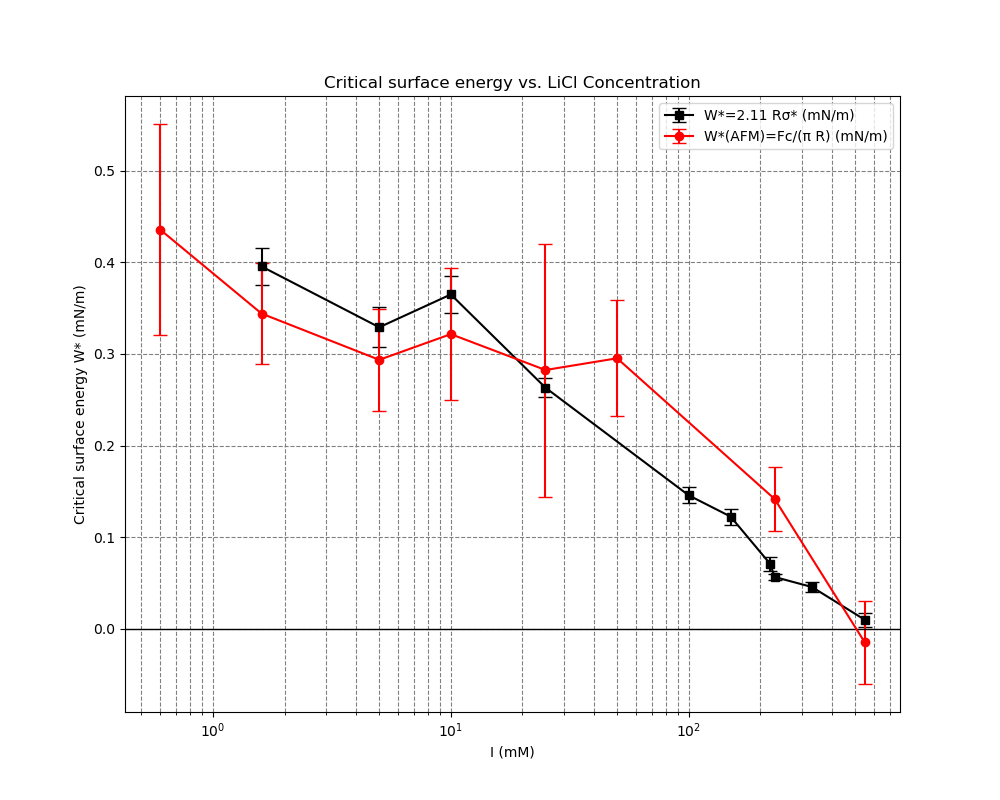
\includegraphics[width=\textwidth]{chapter8/Rheology/Comparison graph.png}
\caption{Critical surface energy values deduced from AFM (red circles) and rheological experiments (black squares) at different ionic strengths.}
\label{fig:critical_surface_energy}
\end{figure}

\section{Comparing results to DLVO theory}


The Force at Contact vs. LiCl Concentration plot is designed to show how the force at the point of contact between an Atomic Force Microscopy (AFM) tip and a sample varies with the concentration of LiCl in a 50:50 water-glycerol mixture. This relationship is important for understanding how ionic strength affects the interaction forces at the nanoscale. In order to examine our results against theory the equations from Chapter 1 were used, which represent general use equations.

\subsection*{Equations Used}

Several equations are used in the script to model the interactions. These equations draw from chapter 1 to represent the types of equations used by those looking to model interactions. Appropriate equations were used to model sphere-plane interactions. 

\textbf{Debye Length:} The inverse Debye length, $\kappa$, is given by
    \[
    \kappa^{-1} = \sqrt{\frac{2 N_A e^2 I}{\varepsilon_0 \varepsilon_r k_B T}},
    \]
    where $N_A$ is Avogadro's number, $e$ is the elementary charge, $I$ is the ionic strength, $\varepsilon_0$ is the vacuum permittivity, $\varepsilon_r$ is the relative permittivity of the mixture, $k_B$ is the Boltzmann constant, and $T$ is the temperature. $\epsilon_r$ was taken from \cite{behrends2006dielectric}
    
\textbf{Electrostatic Repulsion Force:} The electrostatic repulsion force per unit area between a sphere and a plane, taking into account the surface potential $\Psi_0$, is calculated as
    \[
    U_E(r) = 2 \pi R \kappa \epsilon_0 \epsilon_r \left( \frac{k_B T}{e} \right)^2 \tanh^2\left(\frac{e \Psi_0}{4 k_B T}\right) e^{-\kappa h},
    \]
    where $R$ is the radius of the sphere and $h$ is the separation distance. $\Psi_0$ was taken from \cite{silica2021}.
    
\textbf{Van der Waals Force:} The van der Waals force for a sphere-plane interaction is given by
    \[
    U_{\text{vdW}}(r) = -\frac{A_H R}{6 h^2},
    \]
    where $A_H$ is the Hamaker constant taken from \cite{Bergstrom1997}.
    
\textbf{Total Interaction Energy:} The total interaction energy or force at a separation $h$ is the sum of the van der Waals and electrostatic forces. When adjusted for surface roughness, the combined rms roughnesses of the two surfaces was added to the separation distance as a simple means to model roughness.

\begin{table}[h]
\centering
\begin{tabular}{|l|l|}
\hline
\textbf{Parameter} & \textbf{Value (Unit)} \\ \hline
Relative Permittivity, $\epsilon_r$ & 62 (dimensionless) \cite{behrends2006dielectric} \\ \hline
Vacuum Permittivity, $\epsilon_0$ & $8.854 \times 10^{-12}$ F/m \\ \hline
Radius of the Sphere, $R$ & $3.3 \times 10^{-6}$ m \\ \hline
Surface Potential, $\Psi_0$ & -0.040 V \cite{silica2021}\\ \hline
Temperature, $T$ & 300 K \\ \hline
Avogadro's Number, $NA$ & $6.022 \times 10^{23}$ molecules/mol \\ \hline
Elementary Charge, $e$ & $1.602 \times 10^{-19}$ C \\ \hline
Boltzmann Constant, $k_B$ & $1.38064852 \times 10^{-23}$ m\(^2\) kg s\(^{-2}\) K\(^{-1}\) \\ \hline
Separation Distance, $h$ & $2 \times 10^{-9}$ m \\ \hline
Hamaker Constant $A_H$ & $0.63 \times 10^{-20}$ J \cite{Bergstrom1997}\\ \hline
Valency, $z_i$ & 1 (dimensionless) \\ \hline
Roughness Values & $2.4 \times 10^{-10} + 6.45 \times 10^{-10}$ m (chpt 3) \\ \hline
\end{tabular}
\caption{Parameters with their values with units}
\label{table:parameters_units}
\end{table}



\subsection*{Plot Explanation}

The plot displays the calculated force at contact as a function of LiCl concentration. Experimental data points are overlaid to compare the theoretical model with actual measurements. At first figure \ref{fig:calc1} was calculated without the consideration of surface roughness, to gain a baseline.

\begin{figure}[h!]
\centering
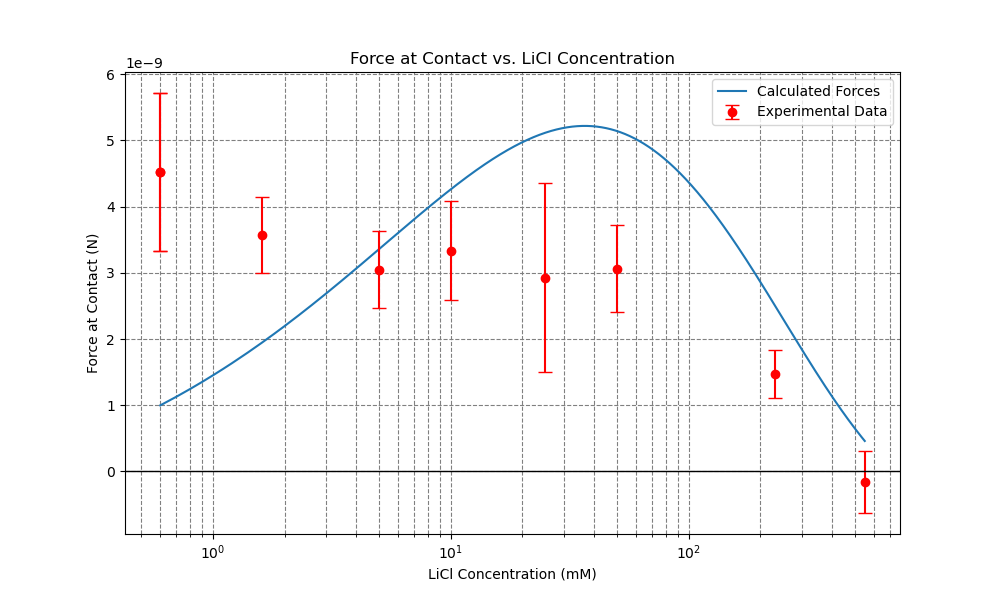
\includegraphics[width=\textwidth]{chapter8/Calculated/No_roughness.png}
\caption{Force at contact from AFM experimental data (red circles) compared against calculated DLVO at different ionic strengths.}
\label{fig:calc1}
\end{figure}

While the calculated fit in figure \ref{fig:calc1} doesn't follow the experimentally derived calculations, there are some useful aspects of this calculation. For one, the values are all roughly same order of magnitude, and the curve follows the downwards trend towards the higher concentrations. This deviation isn't entirely unexpected; DLVO has been known to break down at small lengthscales. \cite{Horinek2014}

One aspect that can easily be added is the roughnesses taken from Chapter 3 (0.24nm rms roughness and 0.64583nm rms roughness), which can then be added to the separation distance.

\begin{figure}[h!]
\centering
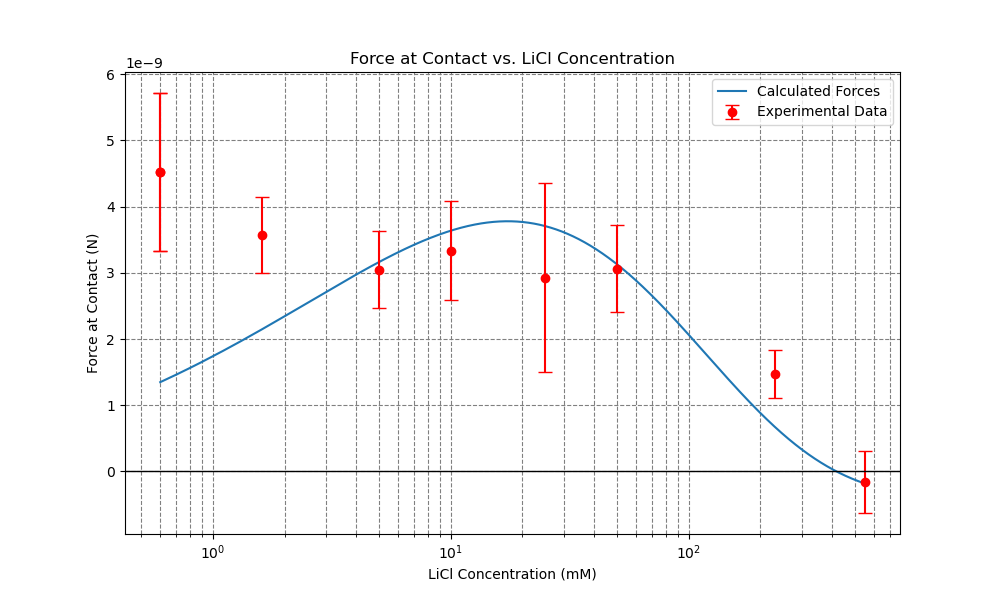
\includegraphics[width=\textwidth]{chapter8/Calculated/roughness.png}
\caption{Force at contact from AFM experimental data (red circles) compared against calculated DLVO with respect to surface roughness at different ionic strengths.}
\label{fig:calc2}
\end{figure}

This addition brings down the curve into a better fit with the experimentally derived data (Figure \ref{fig:calc2}). While this isn't definitive, as there are plenty of other issues with DLVO (such as the inability to predict the shelf seen in both AFM datasets and other papers), it does show that DLVO is sensitive to surface roughness - which we have previously proven to be significantly rough. This trait that could potentially be responsible for the larger degree of variation seen between experimental sites, which could be an avenue worth further exploration.


